\documentclass[border=10pt]{standalone}
\usepackage{tikz}
\usetikzlibrary{shapes.geometric}
\usetikzlibrary{arrows.meta,arrows}
\begin{document}

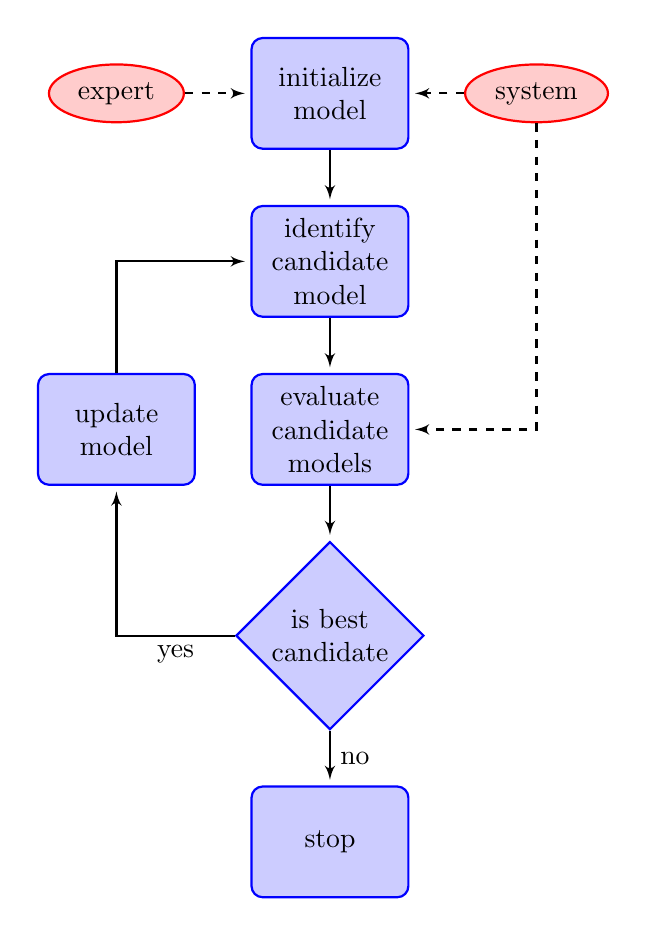
\begin{tikzpicture}
[auto,
decision/.style={diamond, draw=blue, thick, fill=blue!20,
text width=4.5em,align=flush center,
inner sep=1pt},
block/.style ={rectangle, draw=blue, thick, fill=blue!20,
text width=5em,align=center, rounded corners,
minimum height=4em},
line/.style ={draw, thick, -latex',shorten >=2pt},
cloud/.style ={draw=red, thick, ellipse,fill=red!20,
minimum height=2em}]
\matrix [column sep=5mm,row sep=7mm]
{
% row 1
\node [cloud] (expert)      {expert}; &
\node [block] (init)        {initialize model}; &
\node [cloud] (system)      {system}; \\
% row 2
& \node [block] (identify)  {identify candidate model}; & \\
% row 3
\node [block] (update)      {update model}; &
\node [block] (evaluate)    {evaluate candidate models}; & \\
% row 4
& \node [decision] (decide) {is best candidate}; & \\
% row 5
& \node [block] (stop)      {stop}; & \\
};
\begin{scope}[every path/.style=line]
\path (init) -- (identify);
\path (identify) -- (evaluate);
\path (evaluate) -- (decide);
\path (update) |- (identify);
\path (decide) -| node [near start] {yes} (update);
\path (decide) -- node [midway] {no} (stop);
\path [dashed] (expert) -- (init);
\path [dashed] (system) -- (init);
\path [dashed] (system) |- (evaluate);
\end{scope}
\end{tikzpicture}

\end{document} 
